Macrocycles have recently gathered increasing levels of interest in medicinal chemistry. \cite{Driggers2008, Mallinson2012, Dougherty2017, Marsault2011, Abdalla2018, Marsault2017}
Their unique combination of conformationally constrained structure and high level of structural information allows for the design of large, organized structures suitable to interact with extended and featureless binding sites such as those found in protein-protein interactions.\cite{Janin2008, Chène2006, Scott2016, Modell2016} 
Most Food and Drug Administration (FDA)-approved macrocyclic drugs belong to natural products (e.g., erythromycin, tacrolimus) or peptides (e.g., Sandostatin, eptifibatide). \cite{Giordanetto2014}
Peptidic or semipeptidic scaffolds bridge the gap between small molecules and biologics, allying synthetic ease and a broad choice of natural and non-natural amino acids required for rapid and thorough pharmacophoric exploration. 
The main challenge with peptides resides in their physicochemical and pharmacokinetics-absorption, distribution, metabolism, and excretion (PK-ADME) properties. 
While cyclic peptides are typically more stable to proteases compared to their linear counterparts, their high polarity often translates into low bioavailability.\cite{Naylor2017, Fosgerau2015}
Nonetheless, some cyclic peptides cross cell membranes.\cite{Naylor2017, Wang2014, Nielsen2014} 
Developing tools and knowledge to optimize and better predict their structure–permeability relationship is, therefore, a requirement for the field. Such quest found inspiration in studies of the natural cycloundecapeptide cyclosporine A, which is administered orally. 
One prominent structural feature of this natural macrocycle is its high number of N-methylated residues (7 out of 11) and its dynamic structural adaptation to its environment (also known as (aka) chameleonic properties). \cite{Whitty2016, Danelius2020, Witek2017}
The effect of N-methylation on the permeability of cyclic Hexa- and heptapeptides has been systematically investigated since the number and position of N-methylations may be beneficial or detrimental for permeability. \cite{Nielsen2014, Räder2018, White2011, Beck2012, Biron2008, White2011} 

Less explored are the N-alkylated glycines—aka peptoids—in which the side chain has been moved from the $\alpha$-carbon to the amide nitrogen. \cite{Schwochert2015} 
Similar to N-methylation, this modification removes one H-bond donor and removes one stereogenic center and induces glycine-like secondary structures.
The peptoid amide also facilitates cis-trans isomerization compared to the corresponding N-methylation.\cite{Sui2007} 

More recently, the impact of the dynamics of macrocycles in response to their environment, which can range from polar in water, nonhomogeneous in the presence of its target, to lipophilic in the membrane, has been appreciated.\cite{Danelius2020, Witek2017, Riniker2019, Witek2019}
A powerful tool to modulate the properties of peptidic macrocycles is the inclusion of a nonpeptidic tether unit.\cite{Marsault2007, Hoveyda2011, Roux2020} 
This tether can serve multiple purposes: in the context of a target interacting with a specific sequence, various tethers can be screened without modifying the peptide recognition sequence, while providing a simple handle for modulating affinity and PK properties. 
Small modifications in size, shape, or functional groups on the tether can dramatically influence on this kind of constrained system.\cite{Appavoo2019}

The relationship between structure and permeability is known to be elusive for this class of compounds, with small structural modifications often yielding permeability cliffs. \cite{Wang2014, Räder2018, Beck2012, White2011, Roux2020, Bockus2015, Hewitt2015, Rezai2006, Over2016}

To investigate the structural effect of a tether with the length of  5 atoms and the peptide-peptoid change on the compound permeability, our collaborator, synthesized a compound library of 36 molecules. \cite{Comeau2021, Roux2020}

\begin{figure}
    \centering
    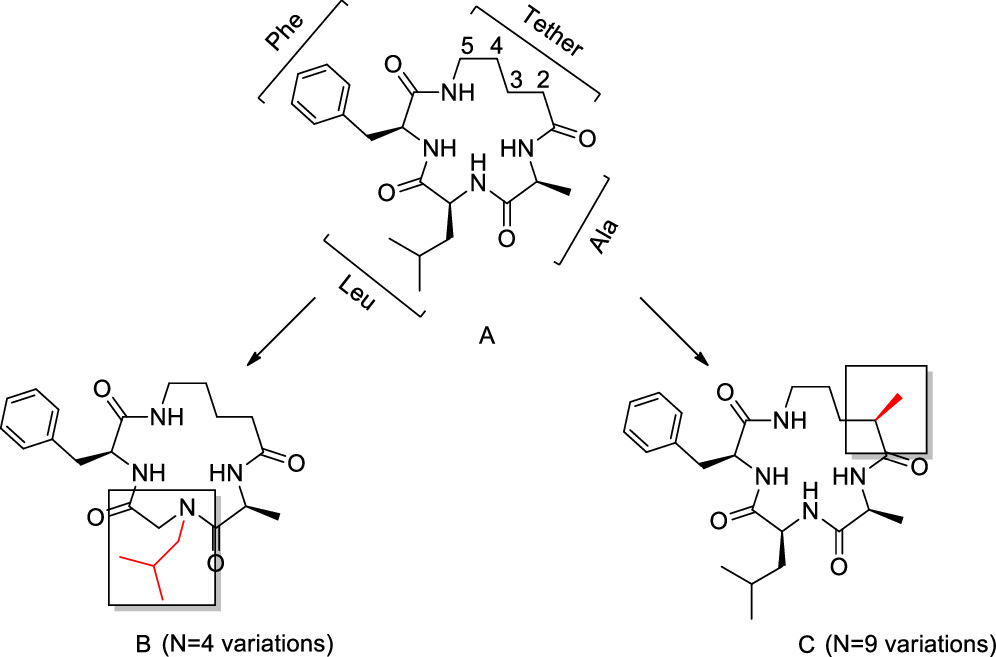
\includegraphics[width=\textwidth]{7_chapter_5/fig/intro/MoleculeDesign.jpeg}
    \caption{Caption}
    \label{fig:MolDes}
\end{figure}

The structure of the compounds was composed of a tripeptide tethered head-to-tail with a nonpeptidic linker (Figure \ref{fig:}). 
Two classes of modifications were implemented on the compounds: single peptoid replacement (B, Figure \ref{fig:}) or regio- and stereocontrolled linker C-methylation (C, Figure \ref{fig:}). 
%

\begin{figure}
    \centering
    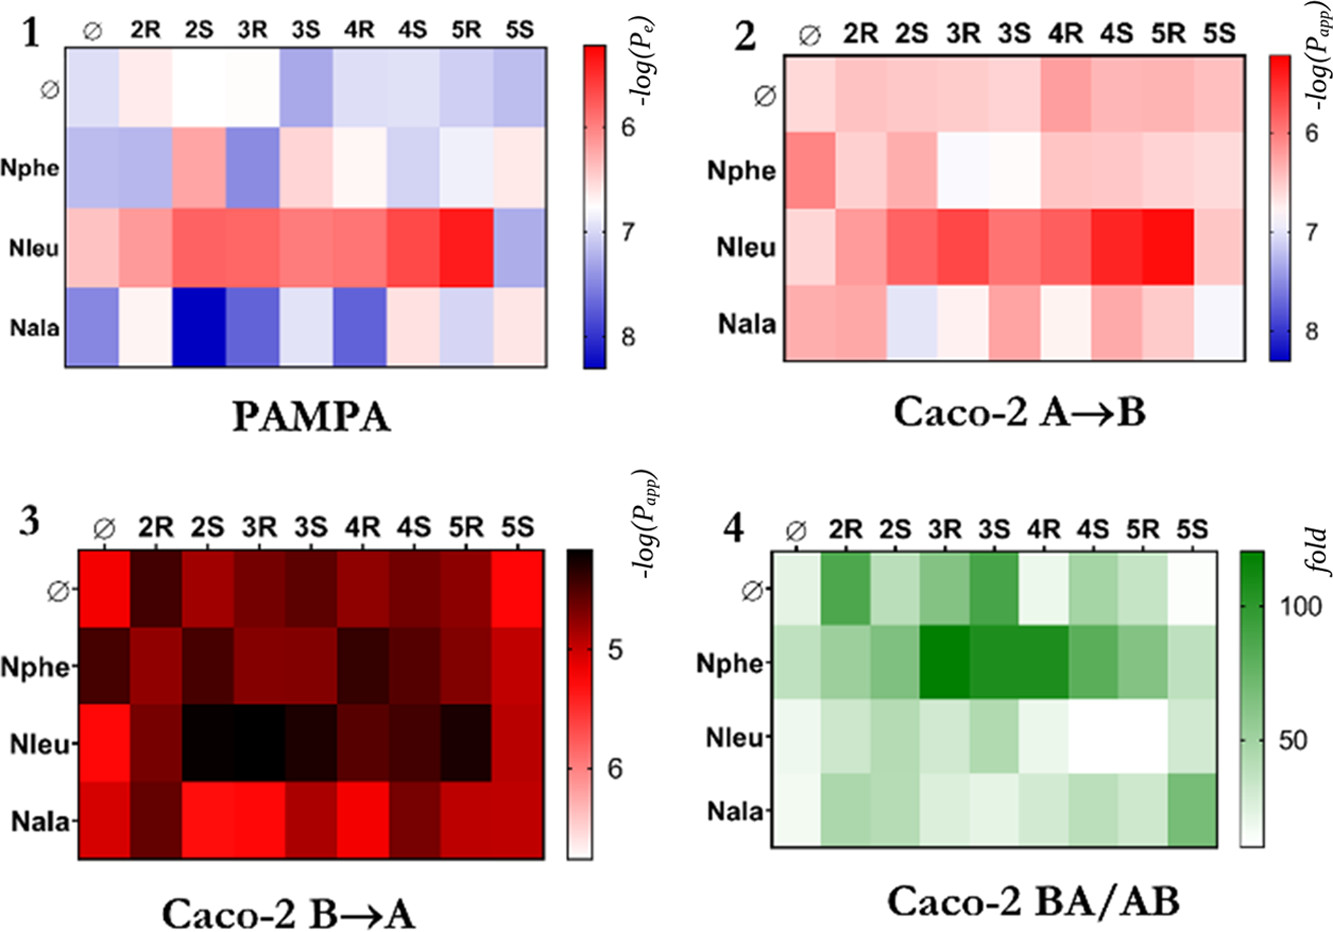
\includegraphics[width=\textwidth]{7_chapter_5/fig/intro/pampa.jpeg}
    \caption{Perm tests}
    \label{fig:permAssays}
\end{figure}

The passive permeability of the resulting macrocycles was measured in the parallel artificial membrane permeability assay (PAMPA) and their cellular permeability in the Caco-2 assay by our collaborator.\cite{Di2015}

%
\begin{figure}
    \centering
    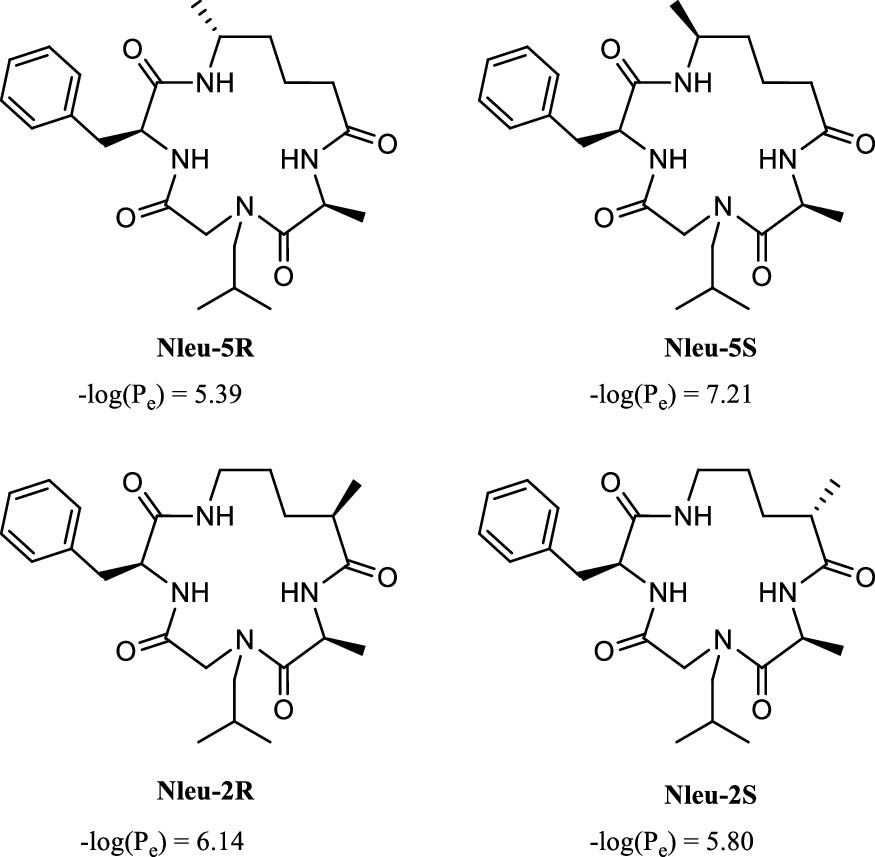
\includegraphics[width=\textwidth]{7_chapter_5/fig/intro/permCliffMols.jpeg}
    \caption{Selected cyclic peptides studied with experimentaQl NMR analysis and molecular dynamics (MD) simulations.}
    \label{fig:permCMols}
\end{figure}
From this data, we selected two pairs of diastereomers that differ only by their stereochemistry of the tether methyl group, yet one pair differs greatly in their passive permeability behavior, contrasted by the second one. 
Prior studies on cyclosporine A showed that the conformational behavior of cyclic peptides in the context of membrane permeability can be studied by setting up simulations in an apolar and a polar environment (i.e., chloroform and water) to study the behavior outside and inside a membrane. \cite{Witek2016,Witek2017, Witek2019, Wang2021}
We, therefore, performed molecular dynamics (MD) simulations of each selected molecule in an apolar and polar environment. Validation of the MD simulations was coupled to solution NMR measurements of the compounds. \cite{Balazs2019}
Finally, we used different metrics to specify the molecules' behavior. The metrics play an important role in explaining the different dynamic behaviors. We explored torsional angles, hydrogen bond formation, and 3D polar surface areas. \cite{Sebastiano2018} 